\documentclass[../main/main.tex]{subfiles}
\begin{document}


\chapter{Zwicky Transient Facility}\label{ch:ztf}

\minitoc
\vspace{2cm}
Nous avons vu dans le chapitre précédent les propriétés
de sonde
cosmologique dont sont dotées les Supernovae de type Ia. Par
ailleurs, nous avons également mis en évidence l'importance de la
classification de ces objets notamment par le biais d'une acquisition
spectrale. Afin d'arriver à cet objectif, la première étape est de
détecter ces évènements transitoires. Dans ce chapitre nous présenterons
la collaboration Zwicky Transient Facility (ZTF par la suite), où la recherche et
l'étude de tels objets sont au centre des activités. Nous nous
focaliserons particulièrement ici sur la section photométrique de
ZTF. Nous commencerons par présenter la collaboration et les raisons de
sa mise en place, puis nous rentrerons dans plus de technicité en
présentant la caméra principale de ZTF et ses capacités
photométriques. Enfin nous parlerons des enjeux cosmologiques et
finirons avec quelques résultats depuis la mise en place de ce grand
relevé astronomique.
\newpage
\section{Presentation de la collaboration}
% \label{sec:xxx}

ZTF ( \citet{GrahamZTF2019} and \citet{BellmZTF2019}) est un grand relevé astronomique dont la première lumière fut
obtenue en Novembre 2017, et réellement actif depuis début 2018. Il
succède au relevé Intermediate Palomar Transient Factory (IPTF, 2012-2017),
lui-même prédécesseur de Palomar Transient Facility (PTF, 2009-2012)
(\citet{RauPTF2009} et \citet{LawPTF2009}). Ces trois relevés grand
champs utilisent le télescope Samuel
Oschin ($48$ pouces $\approx 1m22$) à l'Observatoire de Palomar en
Californie (Fig.~\ref{fig:p48}). D'une caméra avec un champ de vue de $7.9 \text{deg}^{2}$
pour PTF, ZTF utilise à présent pleinement le plan focal du télescope et
bénéficie d'une nouvelle caméra offrant un champ de vue de $47
\text{deg}^{2}$. La collaboration est également doté d'un spectrographe
3D basse résolution ($R\approx100$) monté sur le P48 à Palomar, qui est
utilisé pour suivre les transients détectés par la caméra principale.

\begin{figure}
  \centering
  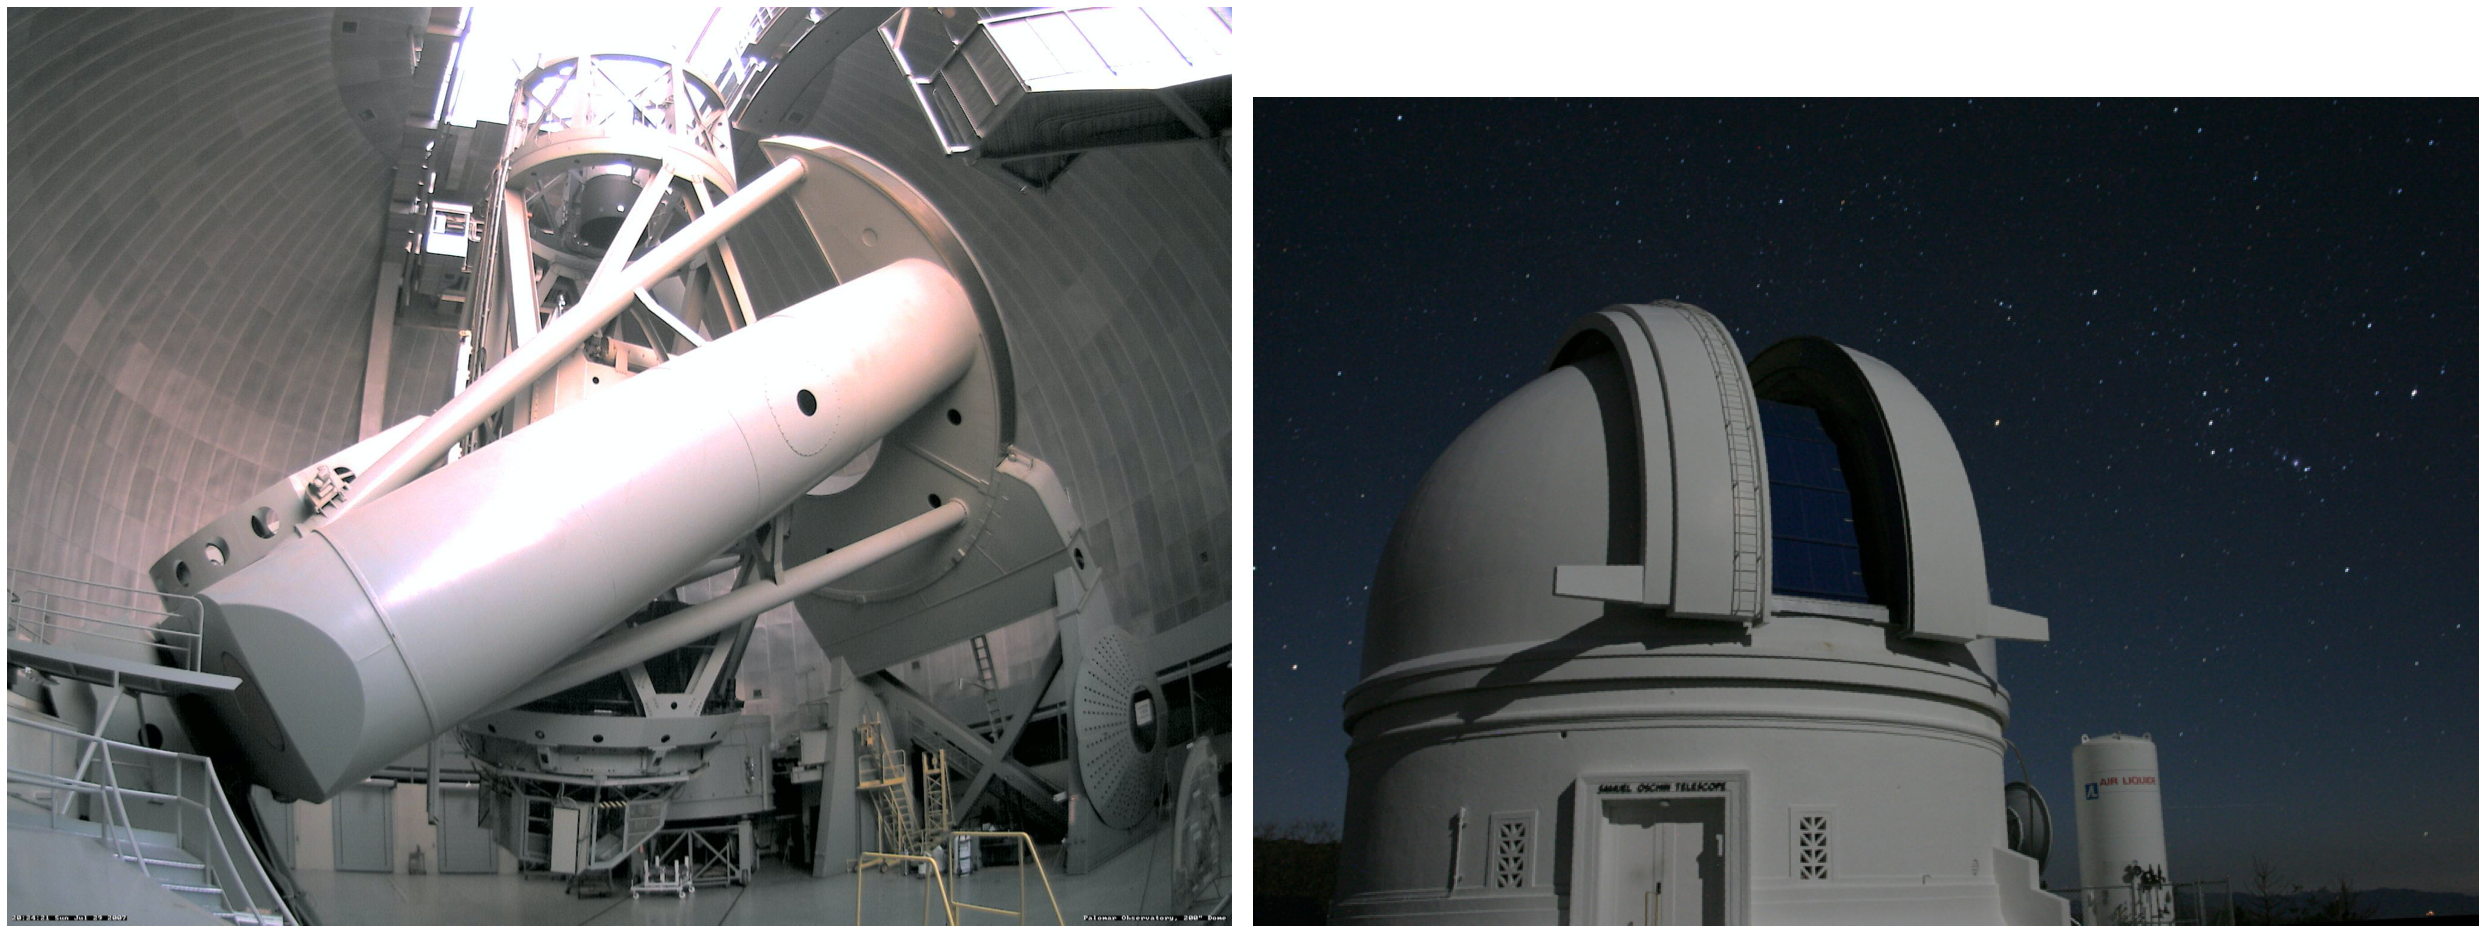
\includegraphics[width=0.75\textwidth]{../figures/02_ztf/p48.png}
  \caption{Télescope Samuel Oshin P48 au Mont Palomar}
  \label{fig:p48}
\end{figure}

ZTF est une collaboration internationale, financée à parts égales entre
la US National Science Foundation et un grand nombre de consortium
internationaux d'Universités et institutions:

\begin{multicols}{2}
\begin{itemize}[noitemsep, label=$\bullet$]
    \item IN2P3\footnote{Institut national de physique nucléaire et de physique
    des particules}.
    \item TANGO University System of Taiwan
    \item Weizmann Institute of Science, Israel
    \item Oskar Klein Center, University of Stockholm, Sweden
    \item DESY/Humboldt University of Berlin, Germany
    \item Ruhr University Bochum, Germany
    \item University of Warwick, UK
    \item Trinity College Dublin, Ireland
    \item University of Maryland, College Park
    \item Northwestern University
    \item University of Wisconsin, Milwaukee
    \item Lawrence Livermore National Laboratory
    \item Caltech/IPAC
\end{itemize}
\end{multicols}

ZTF est ainsi un partenariat privé-public, où son temps d'observation
est divisé entre trois niveaux: le temps d'allocation public (40\%), privé
(interne à la collaboration, 40\%) et une fraction dédiée aux programmes de Caltech (20\%).

Durant le temps d'observation public, ZTF effectue deux relevés distincts: le ciel
Nord d'une part qui est entièrement scanné tous les trois jours dans les
filtres $g$ et $r$, et le plan
Galactique d'autre part, qui lui est entièrement observé chaque nuit
également dans les filtres $g$ et $r$.

Ces deux relevés combinés mènent à la détection et la génération
d'alertes automatiques de plus d'un million d'évènements par nuit. Ces
évènements sont des phénomènes astrophysiques transitoires ou variables,
dont la magnitude de détection est inférieur à $r\approx 20.5$. 

Les sections de recherches scientifiques au sein de ZTF sont nombreuses:

\begin{itemize}[label=$\bullet$]
\setlength\itemsep{1em}
    \item \underline{L'étude des AGN \& TDEs}:
  
      Les AGN sont les Active Galactic Nuclei, des trous noirs
      supermassifs qui accrètent de la matière du reste de la
      galaxie. Les TDEs, ou Tidal Disruption Events, correspondent à des
      phénomènes extrèmement lumineux résultants de cette accrétion de
      matière.

    \item \underline{L'étude des Supernovae comme sonde cosmologique}
      
      Utiliser leur caractéristique de chandelle standardisable pour
      effectuer des mesures précises de distance dans l'Univers
      proche. Avant 2018, seulement $\approx500$ de ces évènements ont
      été observés dans l'Univers proche. En 3 ans ZTF a déterminé près
      de $3000$ distances de ces évènements.

    \item \underline{Physique des Supernovae}

      Indépendamment de leur type, de nombreux mystères demeurent sur la
      physique même de l'explosion des Supernovae. ZTF permet d'obtenir
      un échantillon unique de plusieurs milliers de Supernovae tout
      type confondu qui permet à l'équipe Bright Transient Survey
      (BTS) d'obtenir des mesures non-biaisés de taux de Supernovae, de functions de
      luminosités, de propriétés de galaxies hôte etc.

    \item \underline{Voie Lactée et M31}

      Avec l'observation de plusieurs d'étoiles chaque nuit, tout un
      pôle d'étude s'est formé autour des objets internes à notre
      galaxie, mais également dans la galaxie voisine M31, aka
      Andromède. Cet échantillon gigantesque est utiliser pour étudier
      les naines blanches dont la luminosité varie périodiquement,
      d'autres avec des débris transitoires, les systèmes binaires avec
      émission de rayons-X, et de nombreux autres objets stellaires.


    \item \underline{L'Astrophysique Multimessager}

      Cette toute nouvelle branche a vue le jour notamment grâce aux
      premières détections d'ondes gravitationnelles ou de neutrinos. De
      tels phénomènes sont habituellement grossièrement localisés avec
      la détection de ce type de signal, ce qui rend difficile
      l'identification de la source. Avec son champ de vue extrêmement
      large et sa haute cadence, ZTF est capable de compléter la
      détection primaire avec une observation photométrique aux prémices de
      l'évènement, si une contrepartie électromagnétique existe.

    \item \underline{Corps au sein du système Solaire}

      Ce groupe se concentre sur la découverte et la caractérisation des
      petits corps au sein de notre système solaire, à savoir des
      astéroïdes, des comètes etc.
\end{itemize}



\begin{figure}
  \centering
  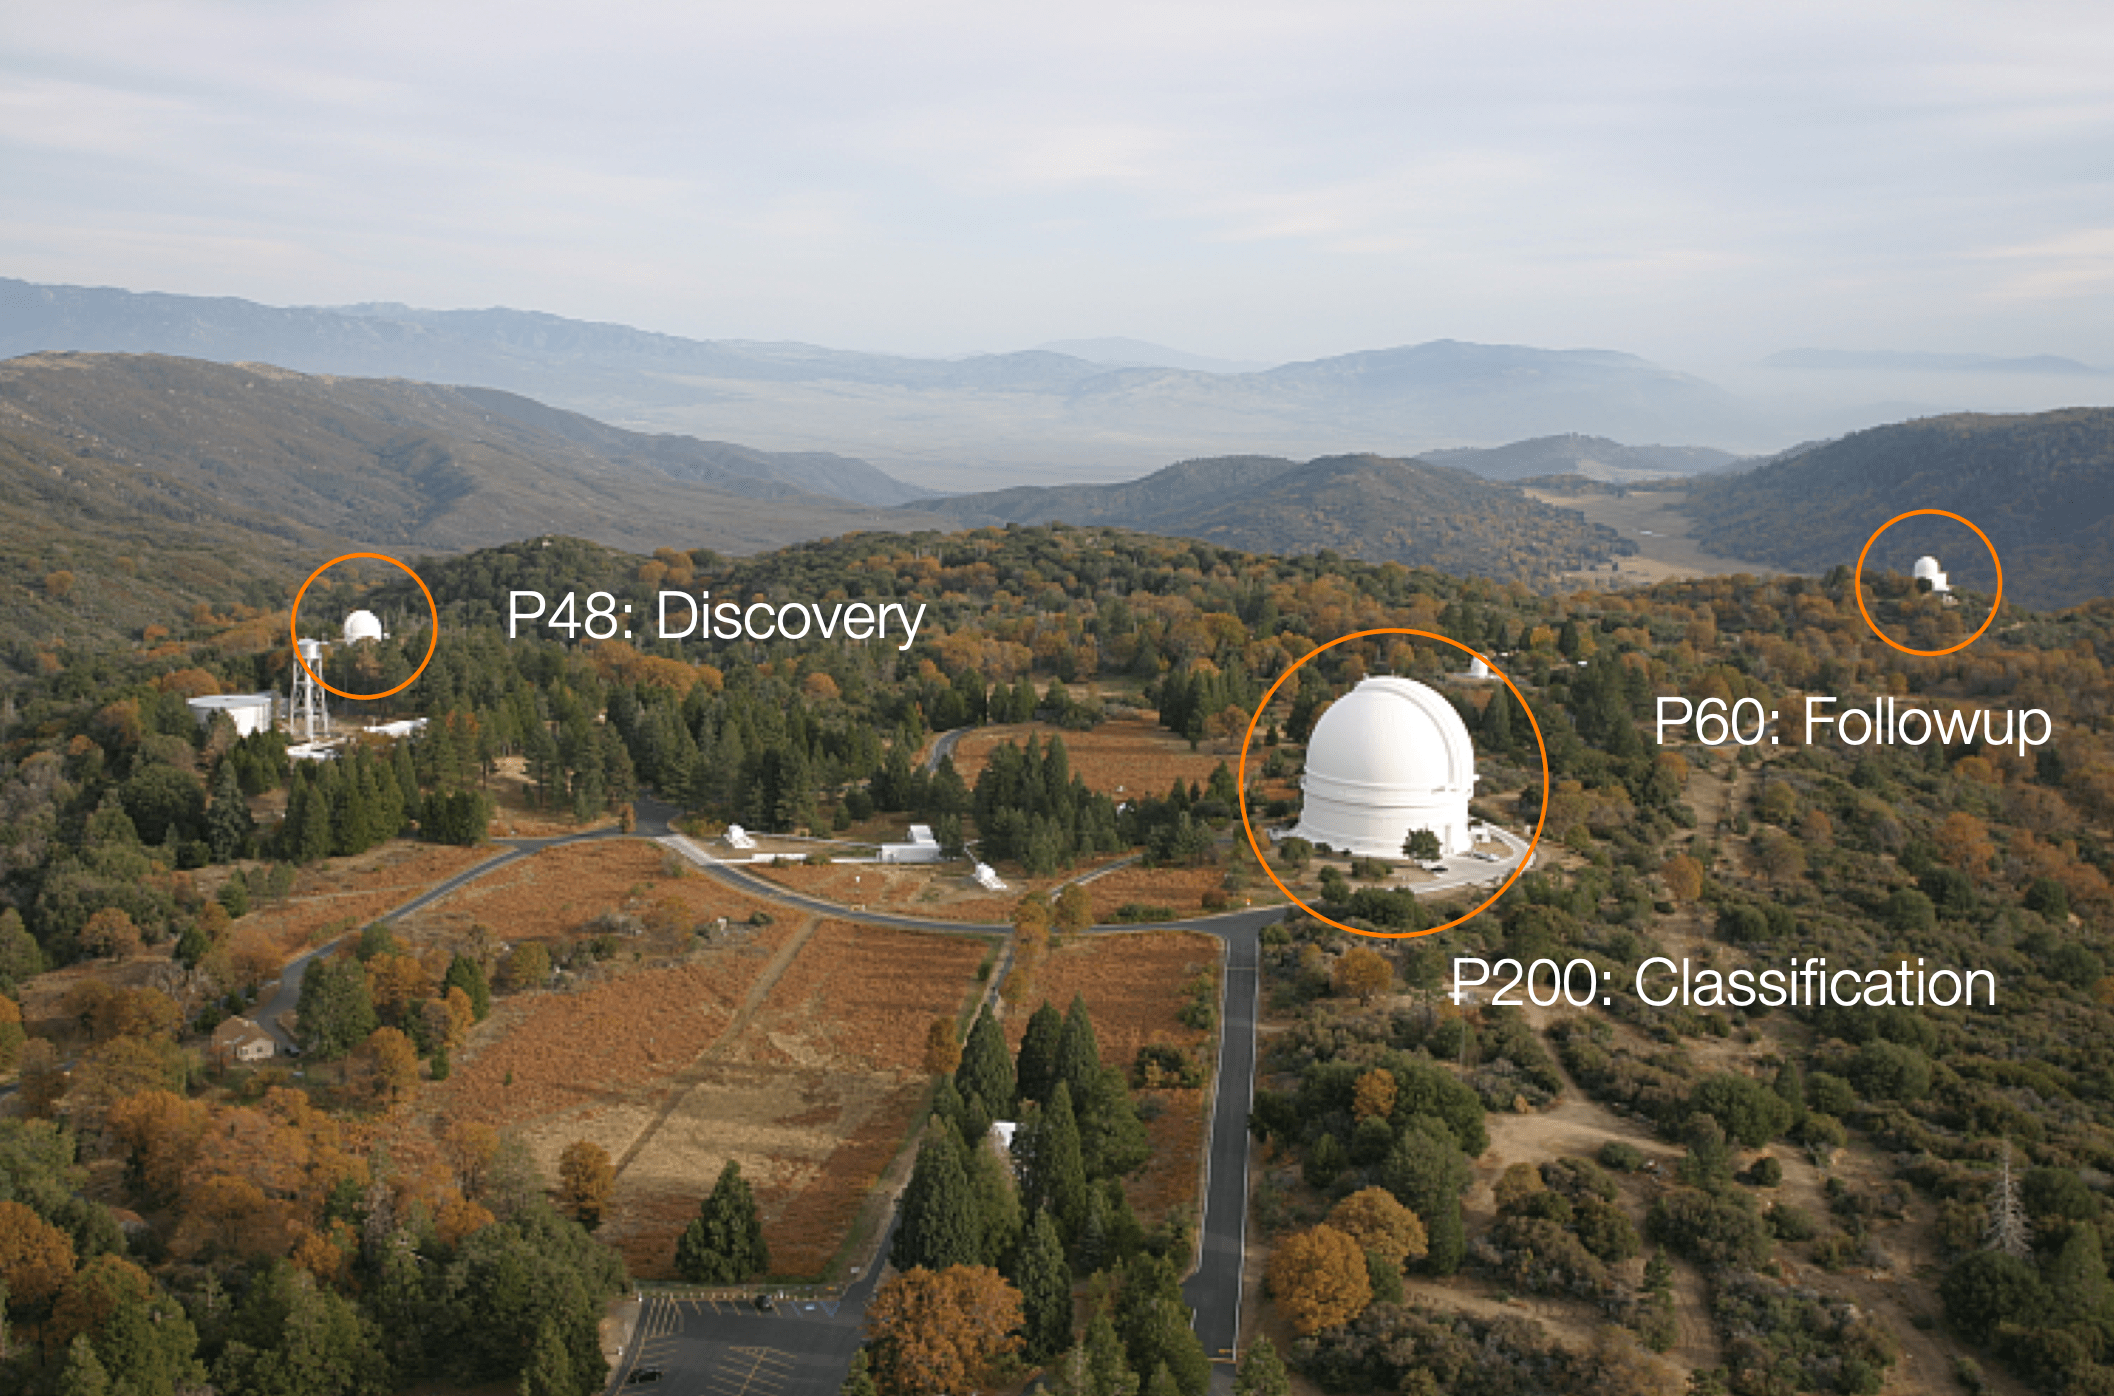
\includegraphics[width=0.75\textwidth]{../figures/02_ztf/palomar_obs-min.png}
  \caption{Observatoire de Palomar, en Californie. Sur la gauche est
    située la caméra principale de ZTF, attachée au télescope P48 Samuel
    Oschi. En haut à droite nous avons le P60, sur lequel est monté le
    spectrographe 3D SEDm appartenant également à la collaboration
    ZTF. Le P200 est quant à lui utiliser par de nombreuses
    collaborations, et est utilisé occasionnellement par ZTF.}
\label{fig:palomar_obs}
\end{figure}

\section{La caméra de ZTF}
% \label{ssec:xxx}

La nouvelle configuration de ZTF vis à vis de ses prédecesseurs PTF/iPTF
est principalement due à sa caméra de $47\text{deg}^{2}$, profitant de
l'intégralité du plan focal du télescope Schmidt P48.

Comme illustré dans la Fig.~\ref{fig:ztfcamera} de \citet{BellmZTF2019}, la caméra est
constituée d'une mosaïque de 16 CCD (Charge Coupled Device) avec des
pixels carrés de \SI{15}{\micro\metre}, à une échelle de $1\farcs01$
$\text{pixel}^{-1}$. La FWHM mediane de la fonction d'étallement du point
(PSF) résultant de cette configuration est de $2\farcs1$ dans les bandes
$g$ et $i$, et de $2\farcs0$ dans la bande $r$. En ce qui concerne la
sensibilité limite en magnitude, la bande $g$ montre un seuil median à
$5\sigma$ de $20.8$mag, la bande $r$ de $20.6$mag et la bande $i$ $19.9$mag.


\begin{figure}[ht]
\centering
\subfloat[Plan focal de la caméra ZTF \citep{BellmZTF2019}.]{\label{fig:ztfcamera}{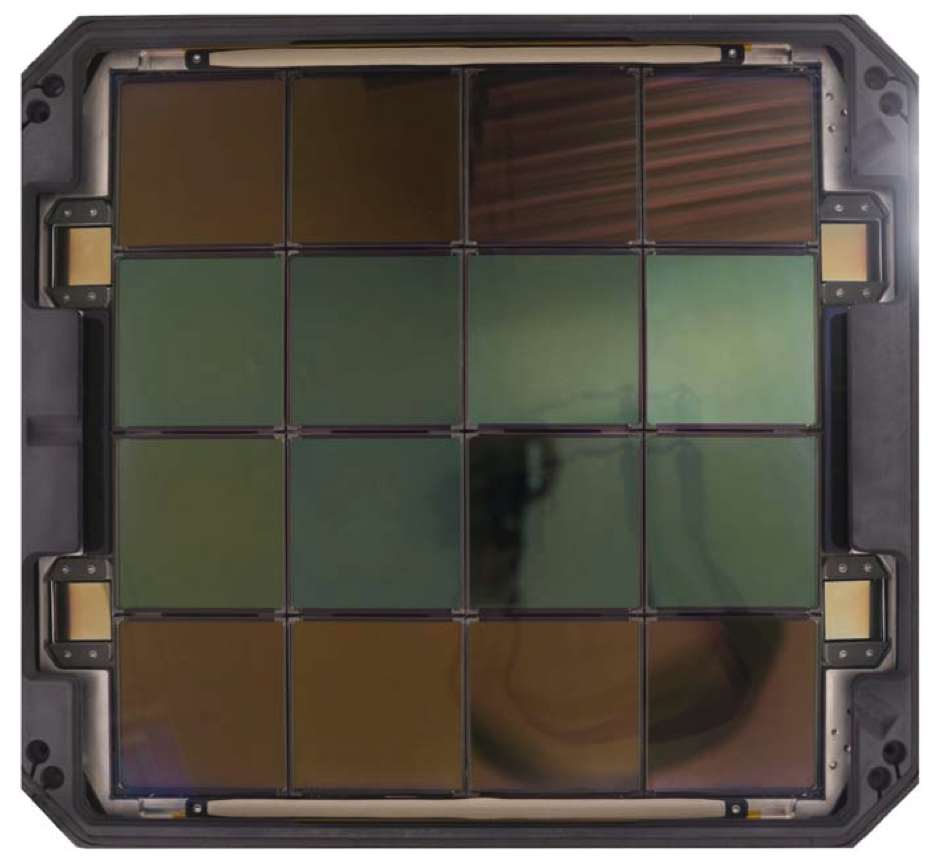
\includegraphics[width=0.4\textwidth]{../figures/02_ztf/ztfcamera.png}}}\hfill
\subfloat[Vue en coupe du télescope Samuel Oschin avec le nouveau
système ZTF \citep{DekanyZTF2020}.]{\label{fig:p48details}{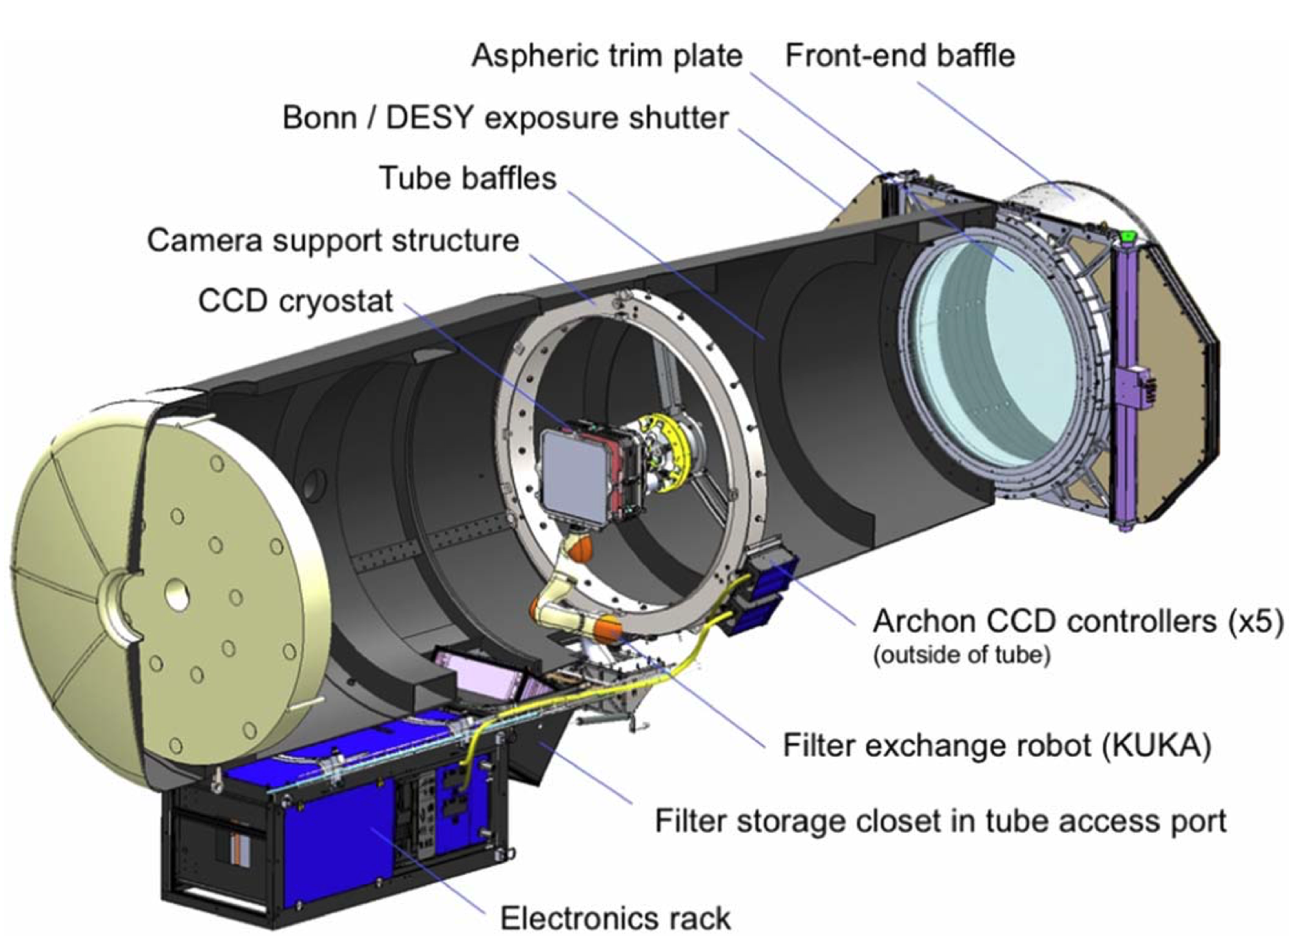
\includegraphics[width=0.5\textwidth]{../figures/02_ztf/p48details.png}}}
\caption{Description du système d'imagerie de ZTF (\textit{à droite}) et présentation du
  plan focal de la caméra et ses 16 CCD (\textit{à gauche}). }
\label{fig:subfigures}
\end{figure}

\begin{figure}
  \centering
  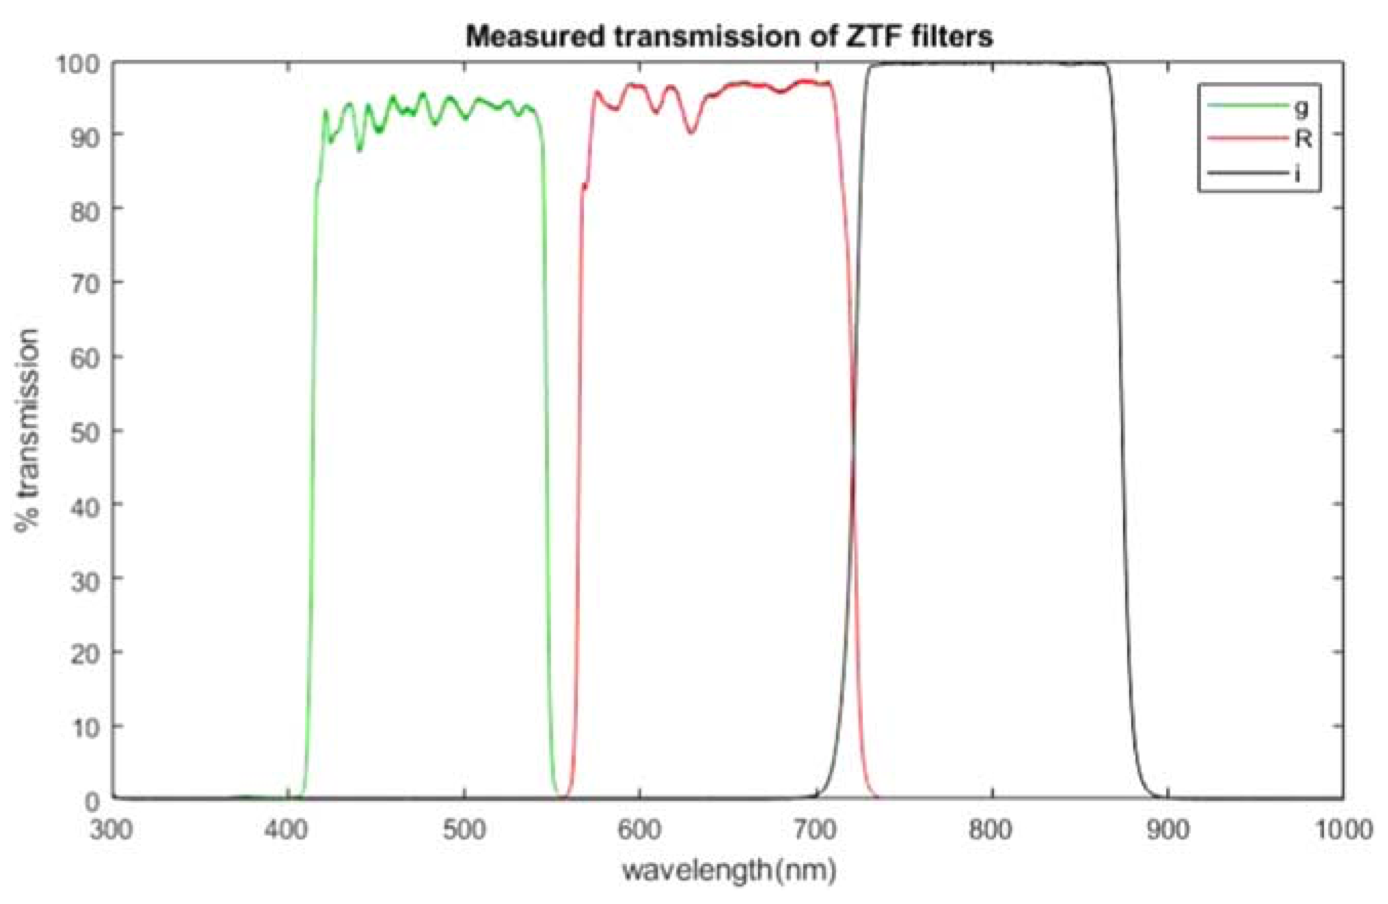
\includegraphics[width=0.75\textwidth]{../figures/02_ztf/ztffilters.png}
  \caption{Transmission des filtres $g$, $r$ et $i$ de la caméra de ZTF \citep{DekanyZTF2020}.}
\label{fig:ztffilters}
\end{figure}


\section{Le rôle de ZTF dans l'étude cosmologique moderne}
%\label{ssec:xxx}

\section{ZTF en quelques chiffres}
%\label{ssec:xxx}


\end{document}

%%% Local Variables:
%%% mode: latex
%%% TeX-master: t
%%% TeX-master: t
%%% TeX-master: t
%%% TeX-master: "../main/main"
%%% TeX-master: t
%%% TeX-master: t
%%% TeX-master: t
%%% TeX-master: t
%%% TeX-master: t
%%% TeX-master: t
%%% End:
